%%%%%%%%%%%%%%%%%%%%%%%%%%%%%%%%%%%%%%%%%%%%%%%%%%%%%%%%%%%%
%%  This Beamer template was created by Cameron Bracken.
%%  Anyone can freely use or modify it for any purpose
%%  without attribution.
%%
%%  Last Modified: January 9, 2009
%%

\documentclass[xcolor=x11names,compress]{beamer}

%% General document %%%%%%%%%%%%%%%%%%%%%%%%%%%%%%%%%%
\usepackage{graphicx}
\usepackage{tikz}
\usepackage[utf8]{inputenc}
\usepackage[spanish]{babel}
\usetikzlibrary{decorations.fractals}
%%%%%%%%%%%%%%%%%%%%%%%%%%%%%%%%%%%%%%%%%%%%%%%%%%%%%%


%% Beamer Layout %%%%%%%%%%%%%%%%%%%%%%%%%%%%%%%%%%
\useoutertheme[subsection=false,shadow]{miniframes}
\useinnertheme{default}
\usefonttheme{serif}
\usepackage{palatino}
\DeclareUnicodeCharacter{00A0}{ }

\setbeamerfont{title like}{shape=\scshape}
\setbeamerfont{frametitle}{shape=\scshape}

\setbeamercolor*{lower separation line head}{bg=DeepSkyBlue4} 
\setbeamercolor*{normal text}{fg=black,bg=white} 
\setbeamercolor*{alerted text}{fg=red} 
\setbeamercolor*{example text}{fg=black} 
\setbeamercolor*{structure}{fg=black} 
 
\setbeamercolor*{palette tertiary}{fg=black,bg=black!10} 
\setbeamercolor*{palette quaternary}{fg=black,bg=black!10} 

\renewcommand{\(}{\begin{columns}}
\renewcommand{\)}{\end{columns}}
\newcommand{\<}[1]{\begin{column}{#1}}
\renewcommand{\>}{\end{column}}
%%%%%%%%%%%%%%%%%%%%%%%%%%%%%%%%%%%%%%%%%%%%%%%%%%




\begin{document}


%%%%%%%%%%%%%%%%%%%%%%%%%%%%%%%%%%%%%%%%%%%%%%%%%%%%%%
%%%%%%%%%%%%%%%%%%%%%%%%%%%%%%%%%%%%%%%%%%%%%%%%%%%%%%
\section{\scshape Introducción}
\begin{frame}
\title{Divide y discriminarás:\\ Una versión distribuída de discriminación de sentidos}
\author{
	Ezequiel Torti López\\}
\subject{Procesamiento de Lenguaje Natural}
\institute{Facultad de Matemática, Astronomía y Física\\Universidad Nacional de Córdoba}
\date{

	\today
}
\titlepage
\end{frame}
%%%%%%%%%%%%%%%%%%%%%%%%%%%%%%%%%%%%%%%%%%%%%%%%%%%%%%
%%%%%%%%%%%%%%%%%%%%%%%%%%%%%%%%%%%%%%%%%%%%%%%%%%%%%%
\begin{frame}
\begin{itemize}
\item Disambiguación de palabras: asignación de sentidos a palabras.
\item Dos subproblemas:
\begin{itemize}
\item Sense discrimination
\item Sense labeling
\end{itemize}
\item Nos concentraremos en Sense discrimination.
\end{itemize}
\end{frame}
%%%%%%%%%%%%%%%%%%%%%%%%%%%%%%%%%%%%%%%%%%%%%%%%%%%%%%
%%%%%%%%%%%%%%%%%%%%%%%%%%%%%%%%%%%%%%%%%%%%%%%%%%%%%%
\begin{frame}
\begin{itemize}
\item Trataré de reproducir el algoritmo de context-group discrimination (Shütze, 1998)
\item Implementa Sense discrimination. No depende de fuentes de conocimiento externas.
\item Aplicaciones:
\begin{itemize}
\item Para algunos problemas de Information Access, sólo es necesario discriminar sentidos.
\item Ej: Similitud y ranking de documentos; dar ejemplos de sentidos de una palabra para una query ambigua.
\end{itemize}
\end{itemize}
\end{frame}
%%%%%%%%%%%%%%%%%%%%%%%%%%%%%%%%%%%%%%%%%%%%%%%%%%%%%%
%%%%%%%%%%%%%%%%%%%%%%%%%%%%%%%%%%%%%%%%%%%%%%%%%%%%%%
\begin{frame}
\begin{itemize}
\item La implementación será sobre un sistema distribuído utilizando Hadoop.
\item ¿Por qué?
\begin{itemize}
\item Buscar una forma de procesar grandes cantidades de datos (hablamos de TB).
\item Hacerlo de forma rápida.
\item Hadoop puede ser útil para algunas cosas \em{si se usa bien}.
\end{itemize}
%Acá hablar sobre que no tengo un corpus de 5 TB, pero dejo sentada una base por si algun dia lo tuviera.
\end{itemize}
\end{frame}

%%%%%%%%%%%%%%%%%%%%%%%%%%%%%%%%%%%%%%%%%%%%%%%%%%%%%%
%%%%%%%%%%%%%%%%%%%%%%%%%%%%%%%%%%%%%%%%%%%%%%%%%%%%%%
\section{\scshape Context-Group Discrimination}
\subsection{Context-Group Discrimination}


\begin{frame}{Context-Group Discrimination}
\begin{itemize}
\item Idea:
\begin{itemize}
\item Inducir sentidos de palabras por las similitudes de los contextos en los que ocurren.
\item La similitud contextual incluso juega un papel crucial en categorización semántica que hacen los humanos.
\end{itemize}
\item Ejemplo:
\begin{itemize}
\item \em{Tenía un vaso de asdf en la mano.}
\item \em{Se le cayó la botella de asdf al piso.}
\item \em{Tomó tanto asdf que al final no podía caminar.}
\end{itemize}
\item ¿Qué es \em{adsf}?
\end{itemize}
\end{frame}

\begin{frame}{Context-Group Discrimination}
\begin{itemize}
\item Idea:
\begin{itemize}
\item Agrupar ocurrencias de palabras en clusters.
\item Cada cluster consiste en palabras con contextos similares.
\item Palabras, contextos y sentidos son representados en un espacio vectorial.
\item Para armar Word Vectors, se observan las coocurrencias de una palabra en una ventana de 50 palabras.
\item Para Context Vectors, se observarán coocurrencias de segundo orden (robustez).
\item Para Sense Vectors, se aglomeran los Context Vectors en clusters y se obtienen sus centroides.
\end{itemize}
\end{itemize}
\end{frame}


\begin{frame}{Context-Group Discrimination}
¿Cómo funciona?
\begin{figure}
\centering
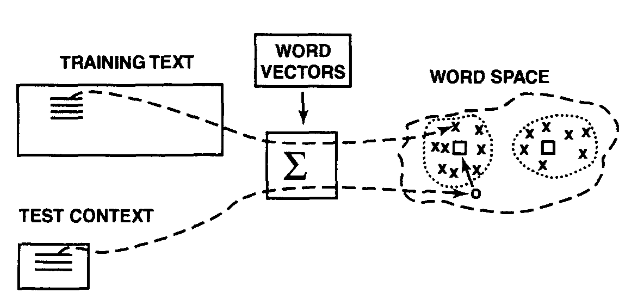
\includegraphics[scale=0.5, keepaspectratio=True, natwidth=800,natheight=600]{basig_design.png}
\end{figure}
\end{frame}

%%%%%%%%%%%%%%%%%%%%%%%%%%%%%%%%%%%%%%%%%%%%%%%%%%%%%%
%%%%%%%%%%%%%%%%%%%%%%%%%%%%%%%%%%%%%%%%%%%%%%%%%%%%%%
\subsection{Word Vectors}
\begin{frame}{Word Vectors}
\begin{itemize}
\item Un Word Vector se construye con los N vecinos de una palabra en el corpus.
\item Una celda I en el vector representa \# veces de coocurrencia de la palabra con la palabra en la posición I.
\item Mientras más overlap haya entre dos vectores, más similiares serán las palabras que representan.
\item ¿Qué palabras usar como dimensiones? Elección: elegir las palabras más frecuentes en el corpus.
\end{itemize}
\begin{figure}
\centering
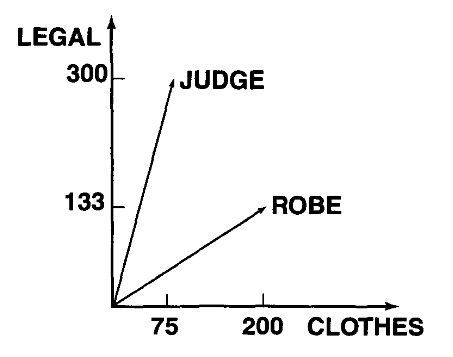
\includegraphics[scale=0.24, keepaspectratio=True, natwidth=800,natheight=600]{word_vector.png}
\end{figure}
\end{frame}

%%%%%%%%%%%%%%%%%%%%%%%%%%%%%%%%%%%%%%%%%%%%%%%%%%%%%%
%%%%%%%%%%%%%%%%%%%%%%%%%%%%%%%%%%%%%%%%%%%%%%%%%%%%%%
\subsection{Context Vectors}
\begin{frame}{Context Vectors}
\begin{itemize}
\item Los WV mezclan sentidos en un solo vector.
\item Necesitamos recorrer el corpus nuevamente, pero esta vez:
\begin{itemize}
\item Analizamos el contexto individual de cada palabra.
\item Sumamos los Word Vectors de las palabras que coocurren = Context Vectors
\end{itemize}
\item Es decir, un Context Vector es un centroide (o suma) de las palabras que ocurren en un contexto.
\end{itemize}
\begin{figure}
\centering
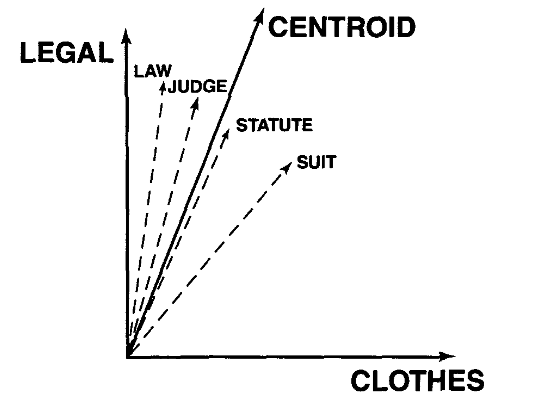
\includegraphics[scale=0.24, keepaspectratio=True, natwidth=800,natheight=600]{context_vector.png}
\end{figure}
\end{frame}

%%%%%%%%%%%%%%%%%%%%%%%%%%%%%%%%%%%%%%%%%%%%%%%%%%%%%%
%%%%%%%%%%%%%%%%%%%%%%%%%%%%%%%%%%%%%%%%%%%%%%%%%%%%%%
\subsection{Sense Vectors}
\begin{frame}{Sense Vectors}
%\begin{itemize}
%\item Son grupos de contextos similares.
%\item Se arman clusters partiendo de TODOS los contextos analizados en el corpus.
%\item Un Sense Vector es simplemente un centroide de cada uno de esos clusters.
%\item Para armar los clusters se utiliza Expectation Maximization.
%\begin{itemize}
%\item Puede converger a soluciones óptimas locales.
%\item Es necesario elegir buenos parámetros iniciales, sino puede converger a minimos locales.
%\item Alternativa: Usar Group-Average agglomerative clustering (GAAC).‎‎
%\end{itemize}
%\end{itemize}
\begin{figure}
\centering
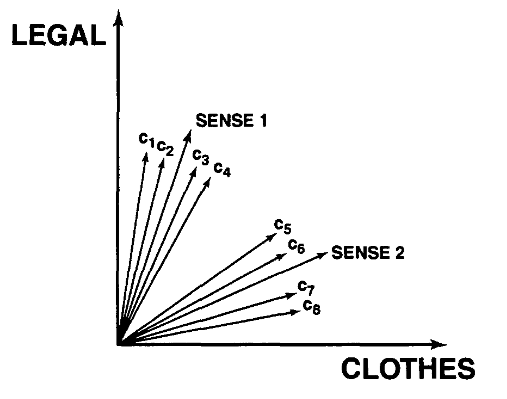
\includegraphics[scale=0.24, keepaspectratio=True, natwidth=800,natheight=600]{sense_vector.png}
\end{figure}
\end{frame}

\subsection{Sense Vectors}
\begin{frame}{Sense Vectors}
\begin{itemize}
\item %Hablar de SVD para una mejor representacion
\end{itemize}
\end{frame}

%Explicar el algoritmo de nuevo con estos nuevos elementos
%Hablar de mis modificaciones (cosas que hice para que el algoritmo sea mas sencillo)
%hablar de haddop
%hablar de la adaptacion a hadoop
%hablar del preprocesamiento y porque convino hacer eso
%Evaluacion (????)


%%%%%%%%%%%%%%%%%%%%%%%%%%%%%%%%%%%%%%%%%%%%%%%%%%%%%%
%%%%%%%%%%%%%%%%%%%%%%%%%%%%%%%%%%%%%%%%%%%%%%%%%%%%%%
\section{\scshape Methodology}
\subsection{frame 1}
\begin{frame}{frame 1}

\end{frame}


%%%%%%%%%%%%%%%%%%%%%%%%%%%%%%%%%%%%%%%%%%%%%%%%%%%%%%
%%%%%%%%%%%%%%%%%%%%%%%%%%%%%%%%%%%%%%%%%%%%%%%%%%%%%%
\subsection{frame 1}
\begin{frame}{frame 1}

\end{frame}

%%%%%%%%%%%%%%%%%%%%%%%%%%%%%%%%%%%%%%%%%%%%%%%%%%%%%%
%%%%%%%%%%%%%%%%%%%%%%%%%%%%%%%%%%%%%%%%%%%%%%%%%%%%%%
\section{\scshape Results}
\subsection{Frame 1}
\begin{frame}{Frame 1}

\end{frame}

\end{document}
